\documentclass[10pt, english, oneside]{article}
\usepackage{geometry}
\geometry{a4paper, margin=.8in}
\usepackage[document]{ragged2e}
%\usepackage[utf8]{inputenc}
\usepackage[english]{babel}
\usepackage{rotating, graphicx}
\usepackage{graphics}
\usepackage{verbatim}
\usepackage{tabularx}
\usepackage{fancyhdr}

\setcounter{secnumdepth}{0}

\pagestyle{fancy}
\fancyhf{}
\lhead{Group 23}
\rhead{Casalino - Gualco - Inglese}
\cfoot{\thepage}

%-------------------------------------------------------------------------------
\begin{document}
% Title
\begin{center}
  \huge \textbf{Low Power Contest}
\end{center}

\justify

%-------------------------------------------------------------------------------
\section{Goal} \label{sec:goal}
The main goal was to provide a tcl script for Synopsys pt\_shell in order to
change the cells exploiting the Dual Vth tecnique.
%-------------------------------------------------------------------------------
\section{Method} \label{sec:method}
Since a change of a cell with the purpose of reducing the power leakage causes a
delay in the circuit, an important effort has been put in the slack: the
algorithm takes the cells in the circuit and analyzes their slack different times.

The algorithm in fact, takes the cells and orders them with respect to the slack
and changes a part of them with the higher slack.
This search, ordering and swapping is done iteratively until the termination of
the algorithm.

The part of them that is changed every iteration corresponds to the number of
the maximum cells allowed to be swapped (given calling the procedure) divided by
a "cycles" factor, that has been calculated in a way that is explained in the
next paragraph and represents the maximum number of swapping cycles.

The swapping loop can finish in two ways:
\begin{itemize}
  \item if there is the soft constraint, it analyzes the slack and, when it detects the
change of the slack from positive to negative, it reverts the cells with HIGHER
o SMALLER slack in the ones just swapped in order to get as close possible with
the required leakage/time tradeoff.
  \item if there is the hard constraint, it loops until the maximum allowed number of
cells has been swapped.
\end{itemize}
%-------------------------------------------------------------------------------
\section{Characterization of the number of cycles} \label{sec:characterization}
The division of the algorithm in different iterations has been seen as a way to
improve the precision of the swapped cells, in order to avoid (especially in the
soft constraint case) a case where is created a new critical path swapping a
series of cells and therefore not exploting well the swapping.

The problem was to decide how many loops the algorithm had to execute. In order
to decide this, it has been explored the space of possibilities: the algorithm
has been tried with different percentages of HVT/LVT cells, with different cycles
(called effort) and has been analyzed the elapsed time and the resulting leakage
power.

Doing so, the resulting data has been analyzed and elaborated with a Matlab
script that is attached in the end of the document.

From this elaboration the effort (number of cycles) decided has been:
\begin{itemize}
  \item hard: 5 cycles
  \item soft: 15 cycles, since it can stop before the end and it means the
    algorithm can try with more effort the cells' swaps.
\end{itemize}

In the next figures it is present the characterization of the soft and hard algorithm.
The red line is the time normalized, the blue is leakage and the yellow is the mean of them.
To estimate the best effort for the screen these graphs has been used.

\begin{figure}[hbt!]
	\centering
	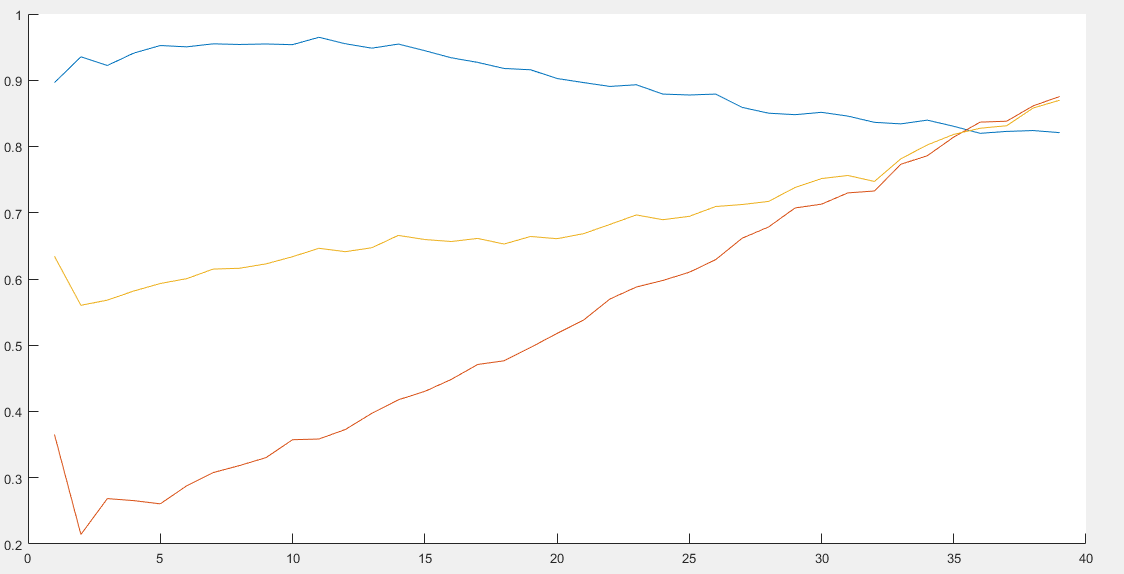
\includegraphics[width=.5\textwidth]{soft.png}
	\caption{Soft characterization}
	\label{fig:soft}
\end{figure}

\begin{figure}[hbt!]
	\centering
	\includegraphics[width=.5\textwidth]{Hard.png}
	\caption{Hard characterization}
	\label{fig:soft}
\end{figure}
\end{document}
